\label{sec:Methods}

* coordinates [limit to nonprecessing?]

* time domain model

* Rather than dwell on relatively well-understood implementation details,  we refer the reader to  Appendix \ref{ap:DiscreteData} for
details of our discrete data handling.

% POINT: Break up the 
As outlined above, we evaluate the posterior probability by reorganiing our


As summarized in Section \ref{sec:Executive}, our algorithm 


\newcommand\itrprm{\vec{\lambda}}
\newcommand\etrprm{\vec{\theta}}

\subsection{Preliminaries}
We begin with the division of the parameter space of compact binary coalescence waveforms. We first define the difference between ``intrinsic'' and ``extrinsic'' parameters. We define $\itrprm$ as the set of intrinsic parameter as those corresponding to the physical configuration of a binary with component masses $m_1$ and $m_2$: $\itrprm=\{\mc,\eta,\Lambda_1,\Lambda_2,\vec{S}_1,\vec{S}_2,\vec{L}\}$, where $\mc$ and $\eta$ are the chirp mass ($(m_1m_2)^{3/5}/(m_1+m_2)^{1/5}$) and symmetric mass ratio ($m_1m_2/(m_1+m_2)^2$), $\Lambda_1$ and $\Lambda_2$ are the tidal numbers of each component mass\footnote{Black holes have no tidal number and thus $\Lambda=0$}, and finally $\vec{S}_1$ and $\vec{S}_2$ correspond to the spin vectors of the component compact objects\footnote{$\vec{L}$, the overall angular momentum of the system is important in the case where the spins are not aligned with the orbital angular momentum, thus causing precession of the orbital plane}. We emphasize in this work rapid determination of source masses --- and possibly compact object type --- thus focusing attention exclusively on $\itrprm=\{\mc,\eta\}$. While the impact of spin and tidal parameters on the waveform are important, they are also potentially complicate the computation of the likelihood in the scheme described later. We thus leave the remaining intrinsic parameters to be built upon in future work.

The extrinsic parameters can be interpreted as the effect of the waveform's arrival and response on a given gravitational-wave detector. For a set of gravitational-wave interferometers, a seven-dimensional space of extrinsic parameters is defined as $\etrprm=\{t_c,\alpha,\delta,\iota,D,\psi,\phi\}$, where $t_c$ is a reference time (usually relative to the geocentric time of coalescence), $\alpha$ and $\delta$ are the right ascension and declination, $\iota$ is the inclination angle of the binary's angular momentum vector and the line of sight to Earth, $D$ is the luminosity distance to the binary\footnote{For the sources considered in this paper, the redshift correction is assumed to be negligible}, $\psi$ is the azimuthal angle of the wave's plane of disturbance to the plane of the arms of the detector, and $\phi$ is the orbital phase of the binary at coalescence. Several subsets of these parameters have well-known (particularly in the non-spinning case) correlations.


\subsection{Background}
%% We reconstruct the parameter

%% \textbf{Concept}* Top-level review: what are we doing (parameter estimation/posterior); establish notation
%% ($\lambda,\theta,L,p,\ldots$)
%% -----



We use Bayes theorem to determine whether the data (denoted symbolically by $\{ d\}$) favors pure noise (hypothesis
$H_0$) or the presence of a signal (hypothesis $H_1$), measured consistently in each of our instruments.  The
gravitational wave signal $h(\lambda,\theta)$ is assumed to have two classes of parameters:
\emph{intrinsic} parameters $\lambda$ (e.g., mass, spin), that fundamentally change the binary's dynamics and hence
gravitational wave signal; and \emph{extrinsic} parameters (e.g., time, distance, sky position), that only change the relative
geometry of the source and our instruments.  Specifically, we evaluate   the odds ratio (or evidence) $Z$:
\begin{align}
\label{eq:def:Z:Modified}
Z(d|H_1) &\equiv \frac{p(\{d\}|H_1)}{p(\{d\}|H_0)} 
%= \int d\lambdap(\vec{\lambda}|H_1)\frac{p(\{d\}|\vec{\lambda},H_1)}{p(\{d\}|H_0)} \nonumber\\
  = \int d\lambda d\theta p(\lambda,\theta|H_1) \Like(\lambda,\theta|\{d\})\ .
\end{align}
where  $p(\lambda,\theta|H_1)$ is our prior probability for the parameters $\lambda,\theta$ (henceforth abbreviated
$p(\lambda,\theta)$ and where $\Like(\lambda,\theta|\{ d\})$ (henceforth for brevity abbreviated $\Like(\lambda,\theta)$) is the likelihood ratio for signal versus noise at the specific parameters
$\lambda,\theta$.  
Similarly, using $x$ to denote all intrinsic and extrinsic parameters except some parameter(s) $y$, we evaluate the marginalized posterior
probability distributions to assess the relative probability density at different values of $y$ given $\{ d\}$:
\begin{eqnarray}
\label{eq:def:Posterior}
p_{\rm post}(y) &\equiv& \frac{\int dx \;  p(y,x|H_1) \Like(y,x)}{ \int d\lambda d\theta p(\lambda,\theta|H_1) \Like(\lambda,\theta)}
\end{eqnarray}
%
Evaluating the above completely generic expressions requires selecting an integration method, a prior,  a signal model, and a
noise model.  


% POINT: Specific details unique to gravitational wave detectors
A standard and extremely effective noise model for gravitational wave parameter estimation is pure gaussian noise.    Following the notation provided in
\cite{gwastro-mergers-HeeSuk-FisherMatrixWithAmplitudeCorrections,gwastro-mergers-HeeSuk-CompareToPE-Aligned}, we
express the likelihood ratio $\Like$ that each interferometer $k$ observed the data $\hat{H}_k(t)$ using our knowledge
of the noise statistics of each instrument.   
%
In this work, we assume each detector has gaussian stationary noise, characterized by a power spectrum $S_k(f)$:
\begin{eqnarray}
\left<\tilde{n}_k(f)^* \tilde{n}_k(f')\right> = \frac{1}{2} S_k(|f|) \delta(f-f')
\end{eqnarray}
where  $\tilde{X}$ denotes the (two-sided) fourier transform of the possibly complex-valued timeseries $X(t)$.  
For each instrument, the power spectrum  defines an inner product between any two timeseries associated with that instrument
\begin{eqnarray} \label{eq:InnerProduct}
\qmstateproduct{a}{b}_k \equiv 2 \int_{-\infty}^{\infty} df \frac{\tilde{a}^*(f)\tilde{b}(f)}{S_k(|f|)}\ .
\end{eqnarray}
In terms of this complex-valued inner product, the likelihood ratio for the data $\hat{H}_k$ can be expressed as
[Eqs. (13-14) of \cite{gwastro-mergers-HeeSuk-CompareToPE-Aligned}]
\begin{align}
\ln \Like(\lambda,\theta) &=
\nonumber -\frac{1}{2} \sum_k \left[ \qmstateproduct{H_k(\lambda,\theta)-\hat{H}_k}{H_k(\lambda,\theta)-\hat{H}_k}_k \right.
\nonumber \\ &  \left. - \qmstateproduct{\hat{H}_k}{\hat{H}_k}_k \right] \nonumber \\
\label{eq:def:LikelihoodRatio}
&=  \sum_k  -\frac{1}{2} \qmstateproduct{H_k(\lambda,\theta)}{H_k(\lambda,\theta)}_k +  \text{Re} \qmstateproduct{H_k(\lambda,\theta)}{\hat{H}_k}_k 
\end{align}
where $H_k(\lambda,\theta)$ is the predicted strain in the $k$th instrument due to a gravitational wave source with
intrinsic parameters $\lambda$ and extrinsic parameters $\theta$.  


% POINT:
In subsequent sections, we will describe the integration method, priors, and  signal model adopted to evaluate
Eqs. (\ref{eq:def:Z:Modified},\ref{eq:def:Posterior}).  

\subsection{Efficiently evaluating the likelihood}

% POINT: Strain formula
The complex gravitational wave strain $h=h_+-ih_\times $ at any sufficiently distant point ($t,\vec{x}$) from a nonprecessing
 binary can be efficiently represented using spin-weighted spherical harmonics $h_{lm}$ as
\begin{align}
\label{eq:h:Expansion}
h(t-\vec{x}\cdot \hat{k}) = \sum_{lm} e^{-2i\psi} h_{lm}(t-\vec{x}\cdot \hat{k})  \Y{-2}_{lm}(\iota,-\phi_c)  \frac{d_{\rm ref}}{d}
\end{align}
where $d_{\rm ref}$ is some reference distance at which the $h_{lm}$ are evaluated.  
In this expression, the vector $\hat{k}$ is the propagation direction ($\hat{k}=-\hat{n}$); the angles $(\iota,\psi)$ are the polar angles of the (fixed) orbital angular momentum direction
relative to the propagation direction $\hat{k}$; $d$ is the distance to the source; and $\phi_c$ is the coalescence
(orbital) phase. 
Expressions for $h_{lm}$ are available in the literature 
\cite{gwastro-pn-MultipoleMomentsNonspinning, gw-astro-mergers-approximations-SpinningPNHigherHarmonics}.  While many
phenomenological approximations do not explicitly provide a harmonic representation, the leading order term ($h_{22}$) can be
easily  identified from published literature by comparing those expressions to the above, evaluated at $\iota=\psi=\phi_c=0$.
  
%
In terms of this complex strain, the response $H_k$ of the $k$th   gravitational wave detector to low-frequency
radiation \cite{gwastro-GroundBasedResponse-Whelan2008} can
be described by a linear combination of $h(t)$ and $h^*(t)$, weighted by time-sky-location-dependent coefficients $F_{+,\times}(t,\hat{n})$:
\begin{align}
H_k(t) &=F_{+,k}(t,-\hat{k}) h_+(t-\vec{x}_k(t)\cdot \hat{k}) \nonumber \\
 & + F_{\times,k}(t,-\hat{k}) h_\times(t-\vec{x}_k(t)\cdot \hat{k}) \nonumber \\
 &=  \frac{F_k(-\hat{k}) h(t-\vec{x}_k(t)\cdot \hat{k}) }{2} + \frac{F_k^*(-\hat{k})h^*(t-\vec{x}_k(t)\cdot \hat{k})}{2}
\label{eq:Hh}
\end{align}
where in the second expression we adopt a complex antenna pattern $F_k=F_{+,k}+i F_{\times,k}$.  
%
For simplicity, in this work we will treat the position $\vec{x}_k$ and antenna pattern $F_k$ of each instrument as
constants.\footnote{The quality of this approximation is in direct proportion to the ratio $|\Delta x|/\lambda$ where
  $\Delta x$ is the change in detector position over the waveform's duration and $\lambda$ is the longest significant
  wavelength.   As either this ratio is a small quantity or the detectors are nearly insensitive to $\lambda$,
  rotation often need not be included.  Moreover, when radiation \emph{does} need to be included, we anticipate a straightforward perturbative and stationary phase
  approximation can augment the simple procedure described above, allowing the likelihood to be well approximated with
  a factor few additional filters and scalars.
}


Substituting this expansion for $h$ [Eq. (\ref{eq:h:Expansion})] and the individual-detector response
[Eq. (\ref{eq:Hh})] into the
likelihood [Eq. (\ref{eq:def:LikelihoodRatio})], we find the likelihood can be expressed as
\begin{widetext}
\begin{align}
\ln \Like(\lambda; \theta) 
&= (d_{\rm ref}/d) \text{Re} \sum_k \sum_{lm}(F_k(-\hat{k}) e^{-2\psi} \Y{-2}_{lm}(\hat{n}))^* Q_{k,lm}(t-\hat{k}\cdot
x_k)
\nonumber \\
&   -\frac{(d_{\rm ref}/d)^2}{2}\sum_k
\left[
{
 \frac{1}{2}|F_k(-\hat{k})|^2 U_{k,lm,lm'}(\lambda)[\Y{-2}_{lm}(\hat{n})]^*\Y{-2}_{l'm'}(\hat{n})
}
% \right. \nonumber \\ & \left.
 {
+
 \frac{1}{2} \text{Re} V_{k,lm,l'm'} e^{-4i\psi}F_k^2 \Y{-2}_{lm}(\hat{n})\Y{-2}_{l'm'}(\hat{n})
}
\right]
\label{eq:def:lnL:Decomposed}
\end{align}
\end{widetext}
In this expression, we use $\hat{n}$ as shorthand for $(\iota,-\phi_c)$; define the constant, detector-dependent
matrices $U,V$ by 
\begin{subequations}
\label{eq:ComputeRhoViaInnerProductMatrix}
\begin{align}
{ U_{k,lm,l'm'}(\lambda)}& = \qmstateproduct{h_{lm}}{h_{l'm'}}_k \\
V_{k,lm,l'm'}(\lambda)& = \qmstateproduct{h_{lm}^*}{h_{l'm'}}_k  \;
\end{align}
\end{subequations}
and define the \emph{filtered data series} $Q_{k,lm}(t)$ via 
\begin{align}
Q_{k,lm}(\tau) &\equiv \qmstateproduct{{\cal T}_{\tau} h_{lm}}{\hat{H}_k}_k \\
&= 2 \int_{-\infty}^{\infty} \frac{df}{S_k(|f|)} e^{+2\pi i f \tau} \tilde{h}_{lm}(f)^* \tilde{\hat{H}}_k(f) \\
\end{align}
i.e., as the inner product of the timeshifted $h_{lm}$ harmonic [$h_{lm}(t+\tau)\equiv [{\cal T}_\tau h_{lm}](t)$] with the data in the $k$th instrument.


% POINT: This is precomputable
Critically, all intrinsic-parameter dependent terms in   Eq. (\ref{eq:def:lnL:Decomposed}) can be evaluated once for
each $\lambda$.  Having calculated these constants ($U_{k,lm,l'm'},V_{k,lm,l'm'}$) and timeseries ($Q_{k,lm}(\tau)$),
the likelihood can be efficiently evaluated for any choice of extrinsic parameters $\theta$.
%

% POINT: Computational requirements
This procedure offers striking reductions in the total number of floating point operations needed to evaluate the
likelihood.
Given how precisely gravitational wave searches time-localize candidate events, only a \emph{short} stretch of data
surrounding a candidate gravitational wave event will ever be examined in  detail.  Hence, rather than evaluate $\Like$ by operating on long-duration, densely sampled
time- or frequency- series, our expression need only act on constants and a few short arrays.  After minimal preprocessing, the total number of
floating point evaluations needed for any \emph{subsequent} likelihood evaluation at those same parameters $\lambda$ is
dramatically reduced.  

%
Since our method employs no assumptions about the structure of $h_{lm}$, this technique for organizing the likelihood
calculation can be applied to any existing waveform model, including the effective-one-body approximants
\cite{gw-astro-EOBspin-Tarrachini2012,gw-astro-EOBNR-Calibrated-2009}.  
%Unlike reduced-order or interpolation-based methods, no further coding, tuning, or calibration is required.  
Our method requires no  additional model- or detector-dependent development  to achieve this performance improvement.  


\subsection{Integrating over extrinsic parameters}
\label{subsec:extrinsic}

% POINT: General integral form
Because precomputed quantities allow us to efficiently evaluate the likelihood $L(\lambda,\theta)$ as a function of
$\theta$, we first integrate the likelihood $L(\lambda,\theta)$ over all extrinsic parameters $\theta$:
\begin{eqnarray}
\LikeRed(\lambda) = \int \Like(\lambda,\theta) p(\theta) d\theta
\end{eqnarray}
where $p(\theta)$ is our prior over the extrinsic  parameters.  We assume the sources analyzed are randomly-oriented and
randomly distributed in the universe out to $D_{\rm max}=300 \unit{Mpc}$.  
%% \begin{eqnarray}
%% p(d)=  3 d^2/d_{\rm max}^3 \quad d_{\rm max} = 300\unit{Mpc} \\
%% \end{eqnarray}
% POINT: Specific separable prior, sampling priors approach
To be concrete, we evaluate the reduced likelihood $\LikeRed$ by integrating over sky position $\Omega_{\rm sky}$ represented
as right ascension $\alpha$ and declination $\delta$; angular momentum orientation, measured by inclination $\iota$ and
polarization angle $\psi$;  and coalescence phase $\phi_{\rm c}$, using the separable prior implicitly provided by the
following integral:
\begin{eqnarray}
\LikeRed(\lambda) = \int \frac{dt}{T_{\rm window}} \frac{d^2 dd d\Omega_{sky} }{V_{\rm max}} \frac{d \cos \iota d\phi_c}{4\pi} \frac{d\psi}{\pi} \Like(\lambda,\theta)
\end{eqnarray}
%
In this expression and our calculations, we adopt a maximum distance $d_{\rm max}$ (here $300 \unit{Mpc}$) and a time window
$ T_{\rm window}$  (here, $300\unit{ms}$)  surrounding the event.  

% POINT: MC
With the exception of time (described below), we evaluate these integrals and reconstruct the posterior distribution using Monte Carlo integration
\cite{book-mm-NumericalRecipies,peter1978new}.   To establish notation used below, we briefly review the general principles  underlying Monte Carlo
integration.  If $p_s$ is a distribution which is never zero when $p>0$, then 
\begin{eqnarray}
\LikeRed(\lambda) = \int \frac{\Like(\lambda,\theta) p(\theta)}{p_s(\theta)} [p_s(\theta) d\theta]
\end{eqnarray}
% POINT: Integral value and its error
% 
If we draw $N$ random samples $\theta_q$ from $p_s$, we can estimate the value $\hat{L}_{\rm red}$ of $L_{\rm red}$ and its error using the
expectation value and central limit theorems for independent, identically-distributed random variables:
\begin{eqnarray}
w_q \equiv \frac{\Like(\lambda,\theta_q) p(\theta_q)}{p_s(\theta_q)} \\
\hat{{\cal L}}_{\rm red}(\lambda) \equiv \frac{1}{N} \sum_q w_q = \left<w\right> \\
\sigma_{\LikeRed}^2 = \left<w^2\right> - \left<w\right>^2
\end{eqnarray}
% POINT: Recombinable
Being a pure Monte Carlo integral, we can  combine the results of multiple independent draws of $N$ events, even if these
evaluations adopted different sampling prior.  As a result, this approach is highly parallelizable.  
% Combining results from multiple runs: because pure Monte Carlo, can combine results after multiple runs, using formula


% POINT: PDF reconstruction
The weighted samples also provide an estimate of the marginalized one-dimensional cumulative distributions $P(<x)$ at
fixed $\lambda$, where $x$ is one of the extrinsic variables in $\theta$:
\begin{eqnarray}
\hat{P}(<x) \equiv \frac{1}{\sum_q w_q} \sum_q w_q \theta(x-x_q)
\end{eqnarray}
[This formula follows by performing Monte Carlo integration on the parameter volume $<x$, keeping track of overall
  normalization.]  
In the limit of many samples, this discontinuous estimate should converge to a smooth, marginalized posterior distribution.  
% POINT: neff
In the typical case that all samples $x_q$ are distinct, the unique sample with the largest weight corresponds to the
largest discontinuity in $\hat{P}$.  The magnitude of this discontinuity, or equivalently its inverse $n_{\rm eff}$,
provides a practical measure of how reliable we expect this one-dimensional posterior to be:
\begin{eqnarray}
n_{\rm eff} \equiv \frac{\sum_q w_q}{\text{max} w_{\rm q}}
\end{eqnarray}
Equivalently, the ``effective number of samples'' $n_{\rm eff}$ measures how many independent samples produce similar
weights near the largest observed weight.  



%
Unless otherwise indicated, we draw samples using a separable sampling prior $p_s(\alpha) =
\prod_{\alpha}p_{s,\alpha}(\theta_\alpha)$, with each factor $p_{s,\alpha}$ equal to the corresponding prior in that dimension.  Notable exceptions are
distance (either uniformly or adaptively sampled) and sky position (either uniformly, adaptively, or via a skymap), as
described below.
%

% POINT: How many runs?
Currently, we perform $n_{\rm trials}$ ($=10$) evaluations at each mass point, terminating when either $N$ iterations
crosses a threshold ($=10^6$) or to some fixed
$n_{\rm eff}$ threshold ($=1000$), whichever comes first.  
% POINT: Storage
To mitigate storage requirements, we discard  low-weight samples before recording results.  Low-weight samples are identified by sorting  $w_1<w_2<\ldots$;
constructing the cumulative $W_=\sum_{q\le k} w_q$; and discarding all samples with $W_k/W_N<10^{-4}$.  

\subsubsection{Adaptive Monte Carlo integration}

To better concentrate our samples in regions of high significance, we implemented a simple adaptive Monte Carlo procedure, adjusting
the sampling prior based on measured weights $w_k$.   In the long term, we expect to apply more sophisticated adaptive
algorithms, as described in the literature \cite{book-mm-NumericalRecipies,peter1978new}.  For reference, we describe
the specific adaptive algorithm implemented used in this work.


% POINT: Adaptive procedure
Every $n_{\rm chunk}$ samples, we reconstruct the one-dimensional sampling priors in each adapting dimension, using
the last $n_{\rm chunk}\times n_{\rm h}$ samples.    In each dimension ($x$), we subdivide the full range
into $n_{\rm bins}$ equal-length bins $X_\alpha$, then evaluate a tempered, weighted histogram
\begin{eqnarray}
W_\alpha = \frac{\sum_{q} w_q^\beta \theta(x_q\in X_\alpha)}{\sum_q w_q^\beta}
\end{eqnarray}
where $\theta(x\in Y)=1$ if  $x$ is in Y and zero otherwise,  and where $\beta$ is a  parameter to moderate the dynamic
range of $w$, described below.  
%
We then \emph{smooth} the array $W$, convolving it with a uniform distribution $n_{\rm smooth}$ bins across.
%
We generated an estimated discrete sampling prior by average the smoothed array $W$ with a uniform distribution with weight $s$:
\begin{eqnarray}
\hat{W}_\alpha = s W + (1-s)/n_{\rm bins}
\end{eqnarray}
% POINT: Discrete to continuous
Finally, we transformed from this discrete, bin-by-bin representation to a continuous integral by (a) constructing
a one-dimensional sampling prior $p_{s,x}(x)$  by interpolating $W^*/\Delta x$ between bin centers, then (b) constructing the
one-dimensional inverse $P_{s,x}(<x)^{-1}$ by integrating $P_{s,x}'(x)=p_{s,x}(x)$.  
%
The latter process ensures that the samplining prior and inverse CDF used to generate random samples are
self-consistent.   
%


% POINT: Specific choices used here
As configured for this paper, we used $n_{\rm bins}=100, n_{\rm hist}=50,n_{\rm smooth}=10,s=0.1$.  We chose the
tempering exponent using the network SNR $\rho$ reported by the search:
\begin{eqnarray}
\beta = \text{min} \left[ 0.8, 4 \frac{\ln (10 n_{\rm chunk})}{\rho^2} \right]
\end{eqnarray}
This choice attempts to mitigate the large dynamic range of $L$ to a scale comparable to the number of samples used in
each histogram.  
\editremark{We should have changed 10 to nhist...}


%% ---- \editremark{Continue here}

%% * General concept

%% * Specific dimensions adapted

%% * tunings adopted: 100 bins, floor, tempering, history

%% * discard values after burn-in? Not yet....




\subsubsection{Using search results to target specific areas of the sky}

The \BS{} pipeline \cite{gw-astro-Bayestar} rapidly processes the results of a search to identify candidate sky
locations consistent with a gravitational wave event, assuming a nonprecessing source.   
%
This code produces a \emph{skymap}: a discrete [Healpix] grid of sky positions, with relative probabilities for each sky
pixel.  
%
Our code can ingest and use these skymaps,  both to construct sampling prior or physical prior \emph{functions}
$p_s(\alpha,\delta)$ and to generate random samples. 

Specifically, the \BS{} pipeline provides a normalized array  $b_k$  for $n=1\ldots n_{\rm pix}$ with $\sum_k b_k=1$.    
Each array index is associated with a unique sky location $(\alpha,\delta)_k $, covering the sky in equal-area tiles.  
%
% Healpy review: http://planck.oat.ts.astro.it/planck/software_and_manuals/Healpix_1.22/Healpix_intro.pdf
%   npix = 12*nside^2 = 49152     %% 4 Pi/(49152)/(Degree)^2 // N
%   nside = 64 (for us)
Because the sky resolutions used are  significantly finer than the resolving power of gravitational wave detector
networks -- and we are free to adopt a higher resolution, as needed, given the expected signal strength -- 
 for simplicity we adopt a purely discrete sky.  For example, to generate  random sky positions, we generating random integers $k$ consistent with
the skymap's probabilities and converting those random integers to sky positions $(\alpha_k,\delta_k)$.  Conversely, to
generate the two-dimensional PDF consistent with this distribution at a proposed $(\alpha,\delta)$, we look up the
integer $k$ associated with the tile containing $(\alpha,\delta)$, then return $b_k$.  



To be more concrete regarding random sky position generation, each random integer is generated as follows. 
%
Without loss of generality, assume the $b_k$ are sorted in increasing order and calculate the cumulative distribution $B_k
= \sum_{q\le k} b_k$.   Random integers $k$ are generated from random real numbers $x$ via finding
% EQUATION
%   - discrete array index q
\begin{eqnarray}
 B_k/B_{n_{\rm pix}} < x <  B_{k+1}/B_{n_{\rm pix}}
\end{eqnarray}
%* review healpy, bayestar 
In practice, to reduce the need to search the $B_k$ array for each new random sample $x$, we quantize the possible probabilities
using some small scale $\Delta p$ estimated from the skymap, then  precompute a lookup table between $\floor*{x/\Delta
  p}$ and $k$.    \textbf{Chris, please verify the implementation}



%% POINT: Very high SNR: finer skymaps are available, and we can use


\subsubsection{Time marginalization}

* Concept only; see Appendix \ref{ap:DiscreteData} for details



\subsection{Placement over intrinsic parameters}

\begin{figure}
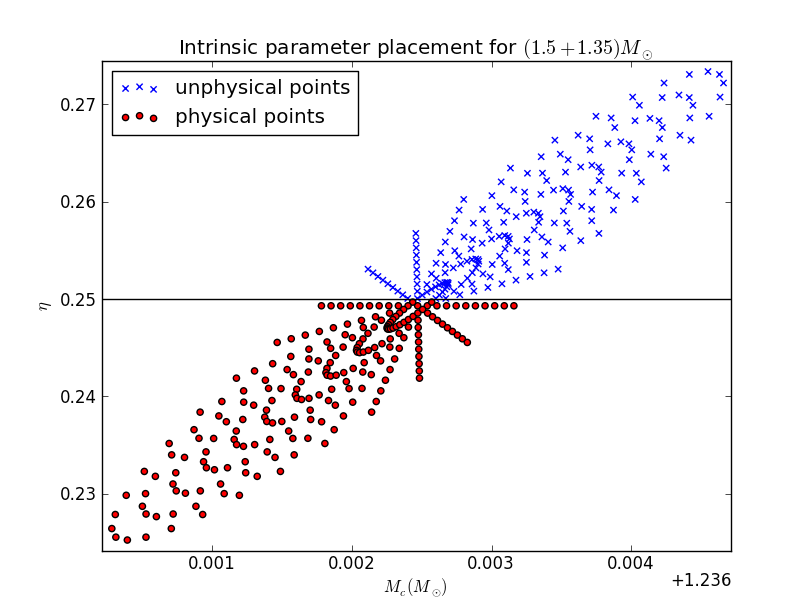
\includegraphics[width=\columnwidth]{../Figures/linear_ellipse_placement.png}
\caption{\label{fig:linear_ellipse} \textbf{Intrinsic parameter placement:} We use an effective Fisher matrix to compute
an approximate ellipsoidal region of overlap $\geq 90\%$ with the masses reported by a detection pipeline.
We then fill this ellipsoid with discrete points and cut any with unphysical values of symmetric mass ratio $\eta$.
At each physical grid point, we marginalize the likelihood over all extrinsic parameters as described in
Sec.~\ref{subsec:extrinsic}.}
\end{figure}

In the current work, we restrict ourselves to considering non-spinning binaries in which we also neglect tidal
effects. Therefore, we need only two mass parameters to describe the intrinsic parameter space, for which we use
the symmetric mass ratio $\eta = m_1 m_2 / M^2$ 
and the chirp mass ${\cal M}_c = M \eta^{3/5}$ (where $M = m_1+m_2$ is the total mass).
Since detection searches will report masses for the candidate event, we use these
to guide which region of the intrinsic parameter space to explore.

Let $\left( {\cal M}^*,\eta^* \right)$ be the masses reported by a detection pipeline. We then perform an effective 
Fisher matrix calculation as described in~\cite{gwastro-mergers-HeeSuk-FisherMatrixWithAmplitudeCorrections,
gwastro-mergers-HeeSuk-CompareToPE-Aligned}
centered about this point.
This involves evaluating the overlap between our waveform with masses $\left( {\cal M}^*,\eta^* \right)$
and $\sim$ tens of nearby waveforms with different intrinsic parameters (while extrinsic parameters are held constant).
The measured overlap values are then fit with a multi-dimensional quadratic. 
The coefficients of this quadratic fit are called the effective Fisher matrix.
Like the standard Fisher matrix, the effective Fisher matrix serves as a quick, crude estimate of expected parameter
estimation performance and can be used to predict surfaces of constant overlap, which will in general be ellipsoids.
In this work, we use the effective Fisher matrix to approximate the region of intrinsic parameter space
which will have overlap $\geq 90\%$ with the masses $\left( {\cal M}^*,\eta^* \right)$.

Once we have defined this $90\%$ overlap ellipsoid, we must fill it with a set of discrete points 
at which we will compute the likelihood. First, we specify the total number of intrinsic parameter points we wish to place,
in this work we used 200 points. Then, these points are arranged within a unit sphere. In this work, we placed
points along 20 radial ``spokes'', with 10 points per spoke. Along each spoke, the points are placed 
uniformly in radial distance. Now, the eigenvalues and eigenvectors of the effective Fisher matrix tell us the lengths
and orientations of the axes of the $90\%$ overlap ellipsoid. We use these to deform and rotate our set
of points in the sphere to a set of points in the $90\%$ overlap ellipsoid.

One subtlety is that the only physically-meaningful values of $\eta$ are in the range $(0, 0.25]$, but the effective Fisher
approach does not account for this physical cutoff. Therefore, for near equal mass binaries where $\eta^* \simeq 0.25$
part of the $90\%$ overlap ellipsoid may have unphysical $\eta$ values. Once we have filled our ellipsoid, we remove
any points that have unphysical $\eta$. To counteract this somewhat, 
we ensure that we always place spokes in our ellipsoid along the direction of constant $\eta$,
so that we always have many points along this boundary of the parameter space.
Fig.~\ref{fig:linear_ellipse} illustrates this placement of intrinsic parameter points.

Note that this intrinsic placement routine could be modified in many different ways. For example, 
we could place points uniformly in volume, rather than uniformly in radius. This would place more points
towards the edge of the ellipsoid, while we chose uniform-in-radius to get more points near the center.
We could also place points randomly inside the ellipse (using uniform-in-volume, uniform-in-radius, 
or any other distribution). We chose the spoked placement so that we can always ensure near-equal mass binaries
will have many points near the $\eta = 0.25$ boundary of the parameter space.
One might also use larger or smaller ellipsoids, use multiple ellipsoids centered at different points if there are concerns
about bias in the masses reported by the detection pipeline, choose points according to a metric, 
or consider any number of other refinements. We plan to refine the intrinsic parameter placement in future work.

\subsection{Postprocessing: intrinsic priors, interpolation, and the final results}

% POINT: Interpolating in intrinsic parameters
At this point, we have evaluated $\LikeRed(\lambda)$ over a structured grid of intrinsic parameters $\lambda_\mu$.  
%
By construction,  the values $\LikeRed(\lambda)$ have small statistical errors (e.g., less than $1\%$).   Using standard
interpolation packages, we interpolate $\LikeRed(\lambda)$ throughout the sampled grid.\footnote{For example, for linear
spoked interpolation in two dimensions, we adopt polar coordinates that are compatible with the 2d polar grid.}
%
Combined with the prior $p(\lambda)$ over intrinsic parameters, we evaluate the overall evidence $Z$ and posterior
distribution $p_{\rm post}(\lambda)$ over intrinsic parameters via
\begin{eqnarray}
Z = \int d\lambda p(\lambda) \LikeRed(\lambda) \\
p_{\rm post}(\lambda) = \frac{1}{Z} p(\lambda) \LikeRed(\lambda)
\end{eqnarray}
%

% POINT: What about posteriors in 
Similarly, we can construct a posterior distribution over some \emph{extrinsic} parameter $x$ by averaging the one-dimensional posterior estimates derived at
each mass point, weighting each by the prior $p(\lambda)$:
\begin{eqnarray}
P_{\rm post}(<x) = \frac{\int d\lambda P_\lambda(<x) \LikeRed(\lambda) p(\lambda)}{\int d \lambda p(\lambda) \LikeRed(\lambda)}
\end{eqnarray}
This weighted average requires interpolating both $\LikeRed(\lambda)$ and $P_\lambda(<x)$ over all $\lambda$.  


% POINT
\editremark{Lazy, current approximation}
To a good approximation, however, the intrinsic and extrinsic parameter distributions often separate after marginalizing
in time.  In other words, after marginalizing in time, the extrinsic parameter distributions are nearly independent of $\lambda$.  
In that case, the level of caution exercised above is unwarranted:  each individual
extrinsic parameter distribution provides a reliable estimate of the posterior.  As a crude approximation to the posterior distribution $p_{\rm post}(\theta)$, we  simply \emph{combine} all
weighted samples $(x_{\mu,q},w_{\mu,q})$ from all mass points $\mu$:
\begin{eqnarray}
\hat{P}(<x) = \frac{\sum_{q\mu} w_{q,\mu}\theta(x-x_{\mu,q})}{\sum_{q\mu} w_{q\mu}}
\end{eqnarray}
[This expression agrees with the general approach, for a specific prior.]
{\color{blue} Feedback?}


